\documentclass[11pt, a4paper, twoside, openright]{article} %draft

\usepackage{graphicx,color}
\usepackage{amssymb, amsmath, array}
\usepackage{epigraph}
\usepackage[font=small,labelfont=bf]{caption}
\usepackage{listings}
\usepackage{makeidx}



% \epigraphsize{\small}% Default
\setlength\epigraphwidth{8cm}
\setlength\epigraphrule{0pt}



\begin{document}


% Example of title page for the projects carried out within DEDIS
% Copied from lasec 

% Simply include it in your mastex tex file: 
%        % Example of title page for the projects carried out within DEDIS
% Copied from lasec 

% Simply include it in your mastex tex file: 
%        % Example of title page for the projects carried out within DEDIS
% Copied from lasec 

% Simply include it in your mastex tex file: 
%        \input{cover}


% Updated October 2016


\newcommand{\logoepfl}[0]{
  \begin{center}
    
\includegraphics[width=4cm]{logo_epfl_coul.eps}
  \end{center}
  \vspace{0.3cm}
  \hrule
}
\newcommand{\project}[1]{
  \begin{center}
    \large{#1}
  \end{center}
  \vspace{1cm}
}
\newcommand{\department}[1]{
  \begin{center}
    \large{#1}
  \end{center}
}
\newcommand{\lab}[1]{
  \begin{center}
    \large{#1}
  \end{center}
}
\newcommand{\supervisor}[3]{
  \begin{center}
    \begin{normalsize}{
        \bf #1}\\#2\\#3
    \end{normalsize}
  \end{center}
}
\renewcommand{\author}[1]{
  \begin{center}
    \Large{#1}
  \end{center}
  \vspace{0.5cm}
}
\renewcommand{\title}[1]{
  \vspace{3cm}
  \begin{center}
    \huge{#1}
  \end{center}
  \vspace{1.7cm}
}
\renewcommand{\date}[2]{
  \begin{center}
    \normalsize{#1 #2}
  \end{center}
  \vspace{0.5cm}
}


\thispagestyle{empty}




% begin title page
  \logoepfl
  
  \title{Proof of Personhood tokens on the ethereum blockchain}
  
  \author{Hugo Roussel}
  \department{School of Computer and Communication Sciences}
  \lab{Decentralized and Distributed Systems lab}
  \project{Bachelor Project}
  
  \date{December}{2017}

  \begin{center}
    \begin{tabular}{cc}
      \begin{tabular}{p{4.0cm}}
        \supervisor{Responsible}{Prof. Bryan Ford}{EPFL / DEDIS}
      \end{tabular}&
      \begin{tabular}{p{4.0cm}}
        \supervisor{Supervisor}{Linus Gasser}{EPFL / DEDIS}
      \end{tabular}
    \end{tabular}
  \end{center}
  

  

% end title page




% Updated October 2016


\newcommand{\logoepfl}[0]{
  \begin{center}
    
\includegraphics[width=4cm]{logo_epfl_coul.eps}
  \end{center}
  \vspace{0.3cm}
  \hrule
}
\newcommand{\project}[1]{
  \begin{center}
    \large{#1}
  \end{center}
  \vspace{1cm}
}
\newcommand{\department}[1]{
  \begin{center}
    \large{#1}
  \end{center}
}
\newcommand{\lab}[1]{
  \begin{center}
    \large{#1}
  \end{center}
}
\newcommand{\supervisor}[3]{
  \begin{center}
    \begin{normalsize}{
        \bf #1}\\#2\\#3
    \end{normalsize}
  \end{center}
}
\renewcommand{\author}[1]{
  \begin{center}
    \Large{#1}
  \end{center}
  \vspace{0.5cm}
}
\renewcommand{\title}[1]{
  \vspace{3cm}
  \begin{center}
    \huge{#1}
  \end{center}
  \vspace{1.7cm}
}
\renewcommand{\date}[2]{
  \begin{center}
    \normalsize{#1 #2}
  \end{center}
  \vspace{0.5cm}
}


\thispagestyle{empty}




% begin title page
  \logoepfl
  
  \title{Proof of Personhood tokens on the ethereum blockchain}
  
  \author{Hugo Roussel}
  \department{School of Computer and Communication Sciences}
  \lab{Decentralized and Distributed Systems lab}
  \project{Bachelor Project}
  
  \date{December}{2017}

  \begin{center}
    \begin{tabular}{cc}
      \begin{tabular}{p{4.0cm}}
        \supervisor{Responsible}{Prof. Bryan Ford}{EPFL / DEDIS}
      \end{tabular}&
      \begin{tabular}{p{4.0cm}}
        \supervisor{Supervisor}{Linus Gasser}{EPFL / DEDIS}
      \end{tabular}
    \end{tabular}
  \end{center}
  

  

% end title page




% Updated October 2016


\newcommand{\logoepfl}[0]{
  \begin{center}
    
\includegraphics[width=4cm]{logo_epfl_coul.eps}
  \end{center}
  \vspace{0.3cm}
  \hrule
}
\newcommand{\project}[1]{
  \begin{center}
    \large{#1}
  \end{center}
  \vspace{1cm}
}
\newcommand{\department}[1]{
  \begin{center}
    \large{#1}
  \end{center}
}
\newcommand{\lab}[1]{
  \begin{center}
    \large{#1}
  \end{center}
}
\newcommand{\supervisor}[3]{
  \begin{center}
    \begin{normalsize}{
        \bf #1}\\#2\\#3
    \end{normalsize}
  \end{center}
}
\renewcommand{\author}[1]{
  \begin{center}
    \Large{#1}
  \end{center}
  \vspace{0.5cm}
}
\renewcommand{\title}[1]{
  \vspace{3cm}
  \begin{center}
    \huge{#1}
  \end{center}
  \vspace{1.7cm}
}
\renewcommand{\date}[2]{
  \begin{center}
    \normalsize{#1 #2}
  \end{center}
  \vspace{0.5cm}
}


\thispagestyle{empty}




% begin title page
  \logoepfl
  
  \title{Proof of Personhood tokens on the ethereum blockchain}
  
  \author{Hugo Roussel}
  \department{School of Computer and Communication Sciences}
  \lab{Decentralized and Distributed Systems lab}
  \project{Bachelor Project}
  
  \date{December}{2017}

  \begin{center}
    \begin{tabular}{cc}
      \begin{tabular}{p{4.0cm}}
        \supervisor{Responsible}{Prof. Bryan Ford}{EPFL / DEDIS}
      \end{tabular}&
      \begin{tabular}{p{4.0cm}}
        \supervisor{Supervisor}{Linus Gasser}{EPFL / DEDIS}
      \end{tabular}
    \end{tabular}
  \end{center}
  

  

% end title page






\newpage

\tableofcontents
\newpage
\section{Introduction}


It is difficult to keep a user accountable and anonymous at the same time on internet. Imagine a forum where users wish to share their political views anonymously but still wish to avoid members that don't add value to the discussion. It's always possible to block an anonymous account but the malicious user can create a new one easily. The forum could then decide to block certain IP addresses but once again the member could use a VPN or a different connection. Another solution would be to ask each new member to provide an ID and verify their identity, however the discussion isn't anonymous anymore. \\
We will explain in the following paper a way to reconcile both ideas and one implementation of it : Proof of Persoonhood tokens and the advantages of porting such a system on a public blockchain.



\section{Proof of Personhood tokens}
\subsection{What are Proof of Personhood tokens?}

\epigraph{``Accountable anonymous credentials``}
{--- \textup{Proof-of-Personhood: Redemocratizing Permissionless Cryptocurrencies}}

Proof of personhood tokens associate a real person with a token, thus binding a physical identity with a digital identity. The results can be achieved by combining pseudonym parties and cryptographic tools.
\subsection{Proof of personhond token as an anti-Sybil attack mechanism}
The Sybil attack is a type of attack in reputation systems where a user forges multiple identities in the goal to use them maliciously. PoP tokens, by verifying the uniqueness of each user, are one of the ways websites can counter this type of attack.
\subsection{Pseudonym parties}

The idea behind a pseudonym party is to verify real people and not real identities. A party goes as follows :  attendees meet at a designated location. Each attendee deposits a public key and once done, the key is added to the set of key of other participants. The person then is marked using permanent marker to insure he doesn't deposit twice. Once each attendee had the chance to register, the party ends and the organizers release the final statement of the party : the keyset of all participants along with details of the party. For transparency purposes the party can be recorded. In that case the hash of the tape is added to the final statement. Attendees can then authenticate anonymously by signing a message with a private key corresponding to the public key deposited.

\subsection{Current implementation}
A first PoP token application was created at the decentralized and distributed systems (DEDIS) laboratory at EPFL, on the Skipchain. The service provides commands for organizers and attendees to link to the skipchain and create proof of personhood tokens. Two pseudonym parties were held using the system in Hamburg and Lausanne in 2016 and 2017 respectively.
The goal of the project was to port the current implementation of PoP token on the Ethereum blockchain, for reasons that are explained below.

\subsection{Limitations}
The Skipchain is a private blockchain, meaning that only certified nodes can be added to it. One of the motivation of the project was to port the service to a public blockchain where ultimately it could be useful to more users.

\section{Ethereum}

\subsection{Ethereum, Solidity and smart contracts}
Ethereum is an open-source public blockchain which can perform decentralized computations on the Ethereum virtual machine (EVM). The EVM is a worldwide computer than anyone can use is exchange for a small fee payed in the crypto-currency of the platform, ether. Scripts running on the EVM are called "smart-contracts". They must be written in Solidity, a Turing complete programming language inspired in its syntax by Javascript. Solidity is compiled to bytecode that is then pushed to the EVM.


\subsection{Why use Ethereum?}

\epigraph{The value of a network is proportional to the square of the number of connected users of the system}
{--- \textup{Metacalfe's law}}

The Ethereum platform quickly gained in popularity after its launch. The ecosystem has many tools to interact with the blockchain and to create decentralized applications. It is currently the network with the most nodes making it more secure and less centralized. A public blockchain also provides a greater transparency as every actor can verify with the contract, who interacts and how.
As the ecosystem grows, the technical barrier to entry is driven down, allowing more users to access it.

\subsection{A quick note on testnets}
To help developers, the Ethereum network provides multiples testnets with free test ethers. Each testnet is similar to the main network with minor differences. The testnet used in this project was the Rinkeby network which is considered the most usable and close to the main network.


\newpage



\section{Implementation of Popcontract}
The popcontract is a smart-contract used to organize and store the informations of a pseudonym party. It is modeled by a finite state machine to improve security and reliability.
\subsection{Abstract}
Create a smart-contract that will store the information of a pseudonym party. At the end of the party, the contract is then locked, rendering it immutable. Each user can then refer to it knowing its genuinity.
The second part of the project consisted in making the system interoperable with the current DEDIS implementation to have a clear and easy-to-use interface.


\begin{minipage}{1\linewidth}
 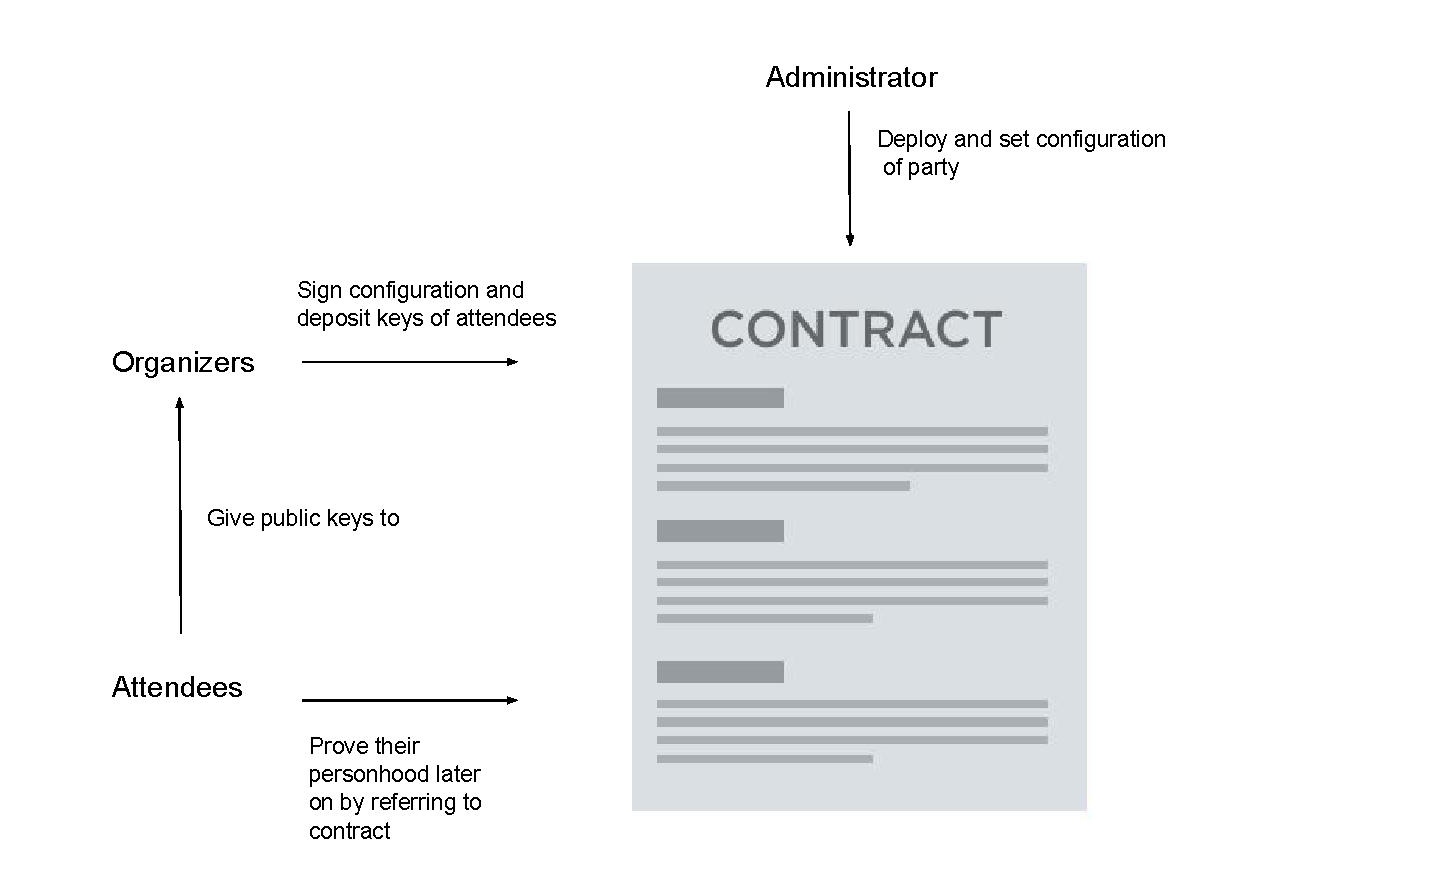
\includegraphics[scale = 0.67]{popcontract.pdf}
 \captionof{figure}{How actors interact with the contract}
\end{minipage}%

\subsection{Popcontract finite state machine}
One of the ways to improve security of a smart contract is to transform it into a finite state machine (FSM). At each state, only pre-defined functions can be called. This reduces the risk that some functions will be called maliciously.\\ The contract is modeled by a FSM with only five states : \\- initial state (contract was succefully deployed)\\ - configurationSet state (administrator provided the details of the party) \\ - configurationSigned state (organizers agreed with the configuration) \\ - key-deposited state (at least one keyset was sent to contract)\\ - locked (party ended and final keyset was choosed)

\begin{minipage}{1\linewidth}
 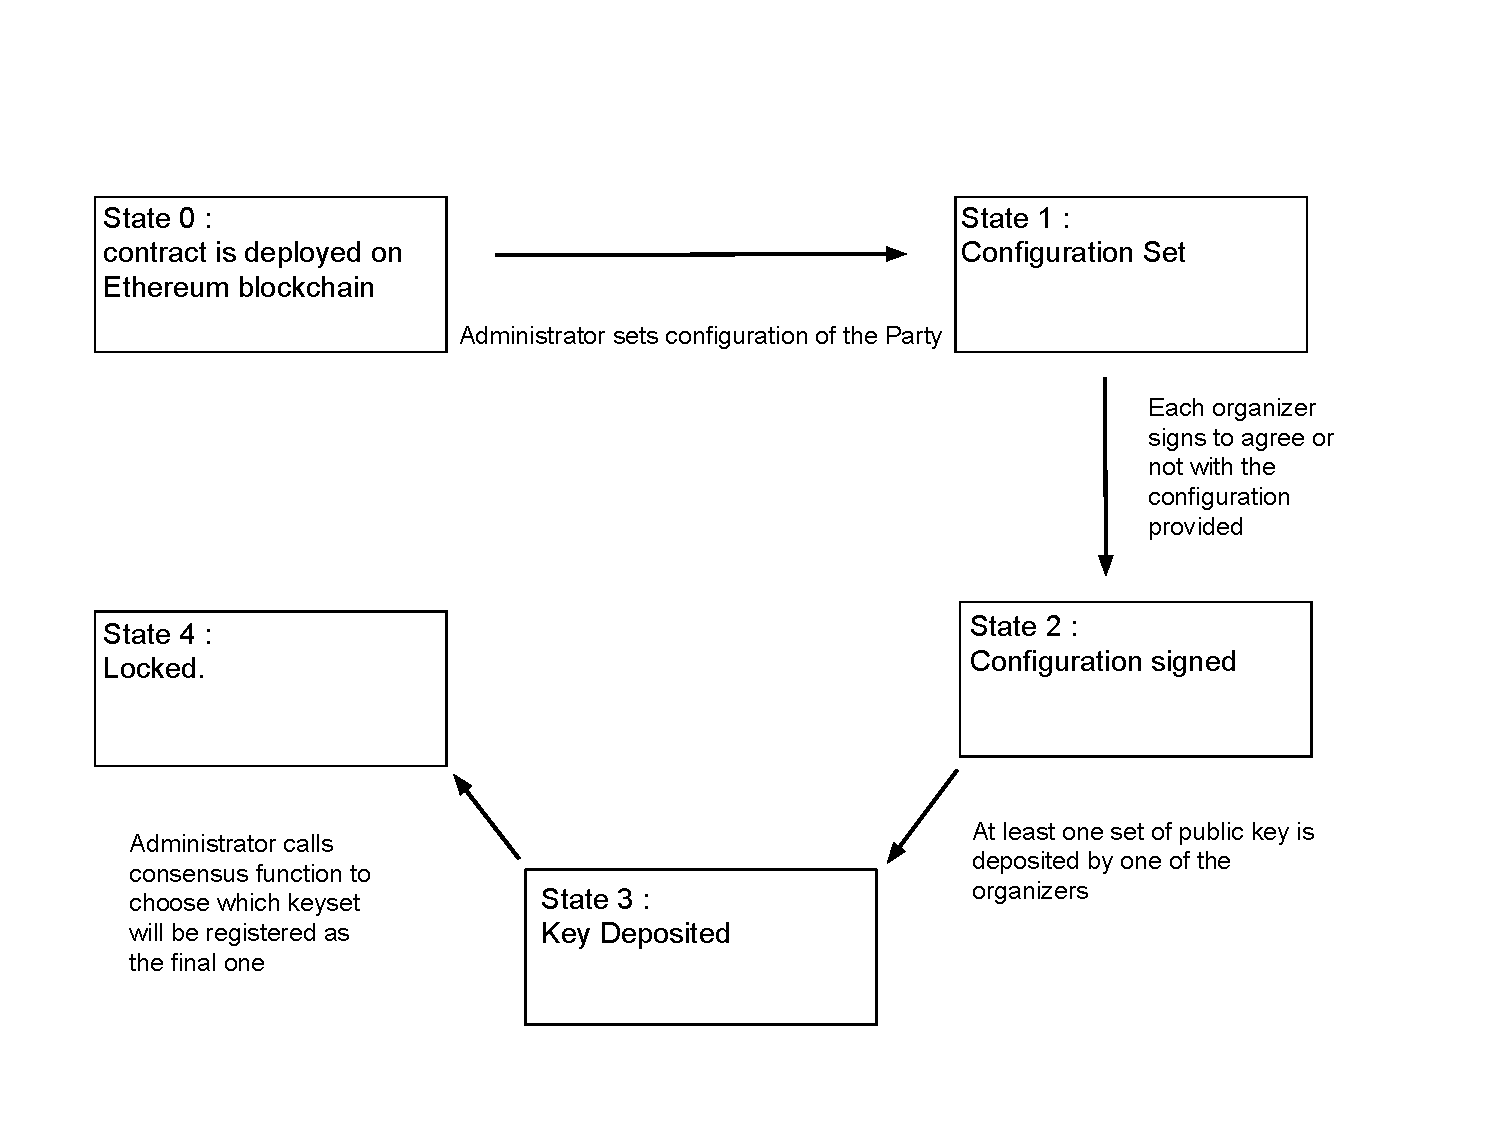
\includegraphics[scale = 0.67]{fsm.pdf}
 \captionof{figure}{Popcontract finite state machine}
\end{minipage}%

\subsection{Technical implementation}
The project focused primarly on the implementation of an application to create PoP tokens, and not in the verification service of attendees personhoods using it.
\subsubsection{Configuration of party}
The configuration of the party is defined as follows : a name, a location, an array of public keys of organizers (in Ethereum format) as well as a deadline. Passed the deadline, no function of the contract is callable, preventing it from being modified. The administrator sends a transaction signed with its private key with all the information above. The administrator is defined as the person holding the private key used to deploy the contract initially. Of course the administrator must have enough ether/test-ether to pay the network fee.
\subsubsection{Signing of configuration}
To prevent a single entity (the administrator) controlling the contract, all the organizers have to sign the configuration by sending a transaction signed with their private key to the contract. As long as the configuration is not fully signed by all organizers, no key can be deposited, and no other function can be called.
\subsubsection{Deposit of public keys of attendees}
The organizers then send a set of public keys to the contract using a transaction signed with their private key including the data they wish to push. The current key type for attendees is compatible with the ed25519 format to allow interoperability with the DEDIS implementation.
\subsubsection{Consensus and lock}
Once at least one keyset is added, the administrator can call a consensus function that will lock the contract and will choose which keyset will be considered as the reference/final keyset.


\subsection{How to interact with an Ethereum smartcontract}
A deployed smart contract is defined by its address and it's ABI (Application Binary Interface). You can get the ABI of a contract using a Solidity compiler. Anyone with these two informations can interact with the contract.
\subsubsection{Creating and sending transactions}
A transaction is a call to the EVM to interact with a contract or an account. Technically a transaction should be from human to human and a message is human to contract or contract to contract. For clarity purposes we will not do the distinction and only use the term transaction. A transaction is constitued of the following fields : \\
- recipient address (contract or human) \\
- signature identifying the sender \\
- value field for transfer of ether. Here this field will always be ignored.\\
- gas limit, the maximum fee the sender is ready to pay \\
- gas price, decided by miners \\
- nonce, the number of transactions made by the account to avoid replay attacks\\
- data field, for a contract this will be the compiled bytecode, for a contract function call, it will be the arguments of the function. \\

It's possible to create raw transactions through a node.js console attached to the network.


\subsubsection{Other ways}
Many tools exist to interact with the ethereum blockchain, we will cite only the most popular ones : \\
- Mist browser, official application that serves both as a wallet and a way to deploy smart-contract and interact with them. You will need to run a full node (download the whole blockchain) to use it or connect to a remote node.\\
- Myetherwallet.com website that serves as a wallet and way to interact with smart contracts. The website is connected to a node and send transactions created on the website to the network. \\
- Metamask, a web browser extension used to deploy and interact with smart contracts. Can hodl ether as well.



\subsection{Interoperability with current system}
Currently the pop implementation at DEDIS uses a command line interface (CLI) to deploy and use the PoP tokens. The goal was to keep the same commands when applicable and create new ones for the new functions.\\The approach taken was to convert the popcontract into a library of golang functions and then integrate those into the CLI application, making it possible to interact with the contract using Golang.\\
The conversion was done using a geth command, called abigen. Geth is a command line interface for running a full ethereum node implemented in Golang. The command takes as input a solidity file and returns a new go file. Everytime the solidity code is modified, type in directory:
\begin{verbatim}
  abigen --sol=popcontract.sol --pkg=main --out=pop.go
\end{verbatim}
This will update the library of go methods in function of the changes to the solidity file.

\section{Theoretical and practical limitations of the implementation.}
\subsection{Theoretical limitations}
\subsubsection*{Scalability}
It might be possible to create large pseudonym parties but after a critical point it becomes highly unpractical for both attendees and organizers to register every member. This might be avoided by doing multiple different parties, which brings new issues. First off, the parties must be held at the same time and sufficiently appart from each other to avoid attendees travelling and depositing multiple keys. Then arises a new issue, how to assure the legitimacy of each organizers of each party? How to assure that attendees don't pay others to use their tokens? How to avoid creation of fake parties? \\ Such issues can be resolved only by trusting the members of the party or complexifying the system.

\subsection{Practical limitations}
\subsubsection*{Adoption and price}
This system is limited by the applications that accept PoP tokens and as such, has very few real use cases on internet. This issue could be resolved by providing a PoP plugin for websites to identify their users with more ease. \\
Another limitation is the barrier to entry for non technical people and their ability to keep their private key safe.\\
Also, if a group of users want to deploy the contract on the main Etheureum network, the fee to deploy can be prohibitive and forces the administrator to buy crypto-currency, a long and tedious process, that might be illegal in some countries. We will address this issue below.
\section{Results}
\subsection{Time to deploy}
The current contract takes on average one minute to deploy. However users don't need to wait until the contract is fully mined to interact with it. During tests, it was shown that sending all transactions with less than one second between them and in order, didn't caused it to malfunction. Each one was mined and activated correctly the contract afterwards. \\
Therefore it is possible to create fully functionnal PoP tokens in less than five minutes.
\subsection{Price in ether}
The current price to deploy the contract is 0.12 eth which is at the current market price is 100 USD at ~840 USD/ETH (coinmarketcap.com the 20/12/2017). It also cost around 19 USD (0.02 eth) to call the heavier functions (configuration setting and key deposit). The price in arguably quite high, but it's noteworthy to mention that high fees were paid to help the contract deploy faster, it might be possible to lower the costs by accepting longer confirmation times. However, since the contract doesn't need value exchange between participants, it can be deployed and used on the testnet for 0 USD.
\section{Possible improvements}

\subsection{Create a friendlier interface}
One of the biggest issues with the current scheme is its difficulty to use for non computer litterate users. It might be interesting to make an app/web-app symplifying the process for attendees and organizers. This could help micro-communities create their tokens with more ease.

\subsection{Improve consensus function and ways to reach it}
The system could be optimized by adding an additionnal parameter in the contract to choose the way the final keyset is choosen. For the moment the contract only returns the last keyset added. There could be different ways to select the good keyset. One example could be voting, where the keyset with the most votes from organizers is selected. Another would be to select the keyset with the least/more keys, or even creating a new keyset with all the different keys added. Optimally, the organizers could sign beforehand the governance system. One of the issues concerning such functions is that computation on the EVM is very expensive and processing the keys is a very heavy process, particurlaly when the keyset becomes large.

\subsection{Size optimization}
If the entity wishing to verify the personhood of participants possess the set of keys, it might be possible to make the contract less expensive to deploy/ more efficient by hashing information. In that way instead of depositing keys, the organizers could push only hashes of the keyset. It is not clear if the efficiency gain is worthwhile compared to the simplicity loss. Optimally the organizers could vote on the preferred type of deposit.

\subsection{Technical improvements}
It could be useful to add a way to choose the key format for attendees. For example adding an ethereum key format choice in the configuration of the contract, this would help attendees use the Ethereum tools.

\subsection{Decrease input parameters}
For the moment the manual input of the nonce is not very practical. Moreover the gas price and gas limit are hardcoded into the app file. Adding a function that would fetch each of those parameters on a reputable website/block-explorer. This would greatly increase practical usability.

\subsection{Better way to handle private keys}
The private key used by the administrator and the organizers is entered in clear and then stocked inside a .conf file. This is not a very secure nor elegant solution.


\section{How to create PoP tokens using the contract}

\subsection{Tools needed to deploy}
\subsubsection*{Geth}
Golang-ethereum, geth, is a command line interface to run a full ethereum node. The installation process can be done using the links provided in the source.
\subsubsection*{Golang}
Golang is a compiled language created by Google. A link is given in the sources for installation.

\subsection{How to deploy a pop contract}
\subsubsection*{Synchronize with the ethereum blockchain}
First you have to run a full node. Depending on the network this will use between 20 and 60 Gb of hardrive space. To synchronize with rinkeby, run :
\begin{verbatim}
geth --rinkeby
\end{verbatim}
Save the path to your geth.ipc file.
The syncing can be long.
\subsection*{Clone the project directory}
Clone the project.
\begin{verbatim}
git clone https://github.com/hugoroussel/popcontract
\end{verbatim}
\subsection*{Create an ethereum account}
Create or use an already existing account. You will need your account ethereum private key and the nonce associated. As mentionned earlier, you can find your nonce by inputing your public address in a block explorer and incrementing the nonce of the last successful transaction. You can also find it directly by running :
\begin{verbatim}
geth attach "your/path/to/geth.ipc"
\end{verbatim}
In the console type :
\begin{verbatim}
eth.web3.getTransactionsCount("public address")
\end{verbatim}
\subsubsection*{Deploy contract}
Go in the cloned directory and run
\begin{verbatim}
go build
\end{verbatim}
This step should not be necessary but will verify that both your go installation and project import went well.
To deploy the contract run :
\begin{verbatim}
./popcontract org link "your private key" "your/path/to/geth.ipc" "nonce"
\end{verbatim}
These parameters will be saved in a configuration file.
The console should show something similar to that :
\begin{verbatim}
hugo@veridisquo:~/popcontract$
./popcontract org link
"3cbae7acc1663d7278bb196eb2fad7aecf465e1560bffc6857d77ed72789a1a3"
"/home/hugo/.ethereum/rinkeby/geth.ipc"
"293"
Successfully linked with : 8347ef6797a784b852021d6806f454affb21e2a3
Transaction receipt :
0e7b84f11d38612cf1acf6a57df03af0beadb66a546e267aad2e1ede004ad3f1
\end{verbatim}



You should normally be able to see in your geth console :
\begin{verbatim}
INFO [12-18|11:03:41] Submitted contract creation
fullhash=0x0e7b84f11d38612cf1acf6a57df03af0beadb66a546e267aad2e1ede004ad3f1
contract=0x8347eF6797A784B852021d6806f454Affb21E2A3
\end{verbatim}
You can use the private key used on the rinkeby network if you wish.
The hash and contract address match the ones above, so everything went well.
As soon as the transaction is mined, your contract is deployed. You can verify it by checking the contract public address in a block explorer, or using the hash of the transaction. Here we can see that the above contract deployment was successful in etherscan.io :
\begin{center}
 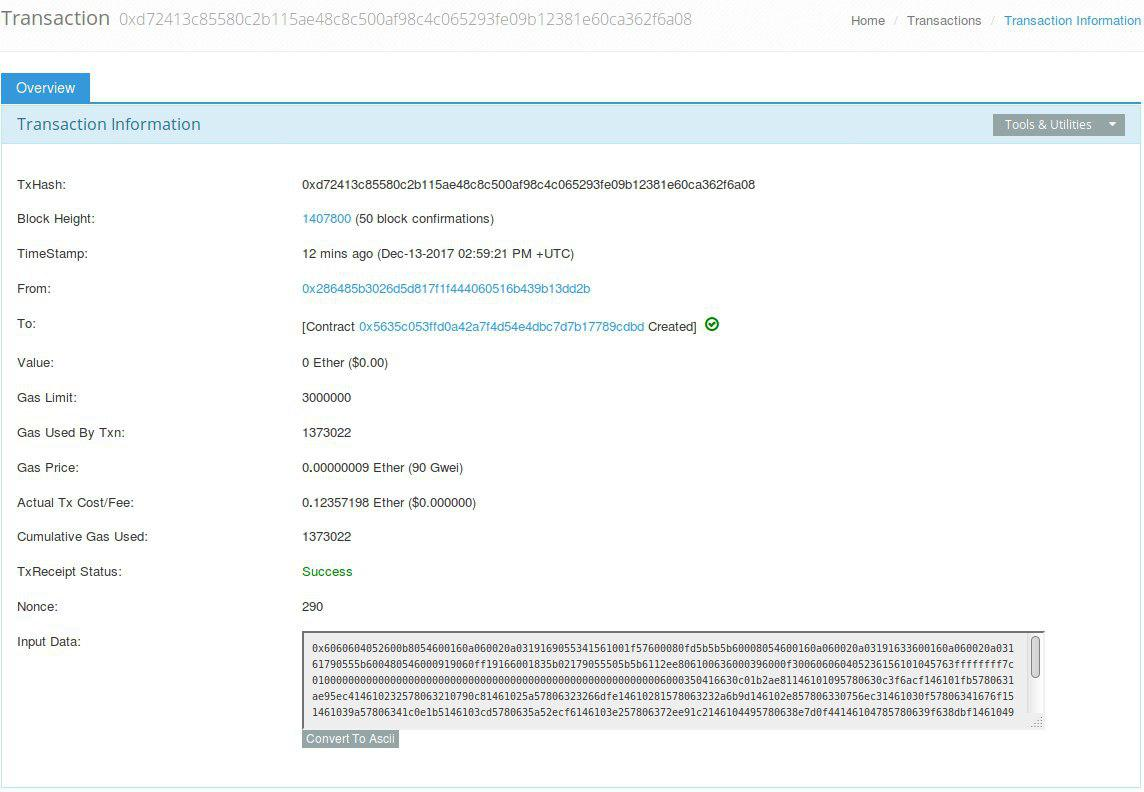
\includegraphics[scale=0.38]{blockexplorer.jpg}
\end{center}
\subsubsection*{Set the configuration of the contract}

To set the configuration of the contract :
\begin{verbatim}
./popcontract org config "desc.toml"
\end{verbatim}
Example of desc.toml file :
\begin{verbatim}
Name = "First party"
Location = "Nazareth"
NumberOfOrganizers = 1
OrganizersAddresses = ["0x286485b3026d5d817f1f444060516b439b13dd2b"]
Deadline = 60
\end{verbatim}
Note : here the organizers and the administrator are the same person, so the contract is controlled by a single entity.\\
The console should display the hash of the transaction. Once again you can verify online that the transaction was successful.

\subsection{How to interact with contract}
To sign the configuration the organizers should run :
\begin{verbatim}
./popcontract org sign
\end{verbatim}
The administrator can then start the key deposit by signing the whole configuration:
\begin{verbatim}
./popcontract org signAdmin
\end{verbatim}
This step verify that all organizers signed the configuration. \\
To deposit new key set :
\begin{verbatim}
./popcontract org public "private key" "keyset"
\end{verbatim}
Note that if a non organizer tries to invoke the function, the transaction will fail.
To reach consensus the administrator calls the following function :
\begin{verbatim}
./popcontract org final
\end{verbatim}
The contract is now immutable, and attendees can use it to authenticate anonymously.
\section{Conclusion}
The use of blockchain technology is particularly interesting in applications where transparency is needed. It applied perfectly to proof of
personhood tokens, as every attendee and organizer can verify the action taken by each other. While being one of the largest blockchain, the Etheurem network is still very new and as such experimental. Creating smart-contract is a relatively straight forward process hindered only by
(sometimes) the lack of documentation and the need to understand the possible attack vectors.\\
On a personal point of view, developing such an application was a very rewarding and enlightning process, which allowed me to discover and put to use the inner workings
of a decentralized network.
\newpage

\section*{References}
\subsection*{Proof of personhood tokens}
\subsubsection*{Original paper by Bryan Ford}
Pseudonym Parties: An Offline Foundation for Online Accountable Pseudonyms
\subsubsection*{DEDIS github PoP project}
https://github.com/dedis/cothority/tree/master/pop
\subsection*{Ethereum documentation}
\subsubsection*{Solidity documentation}
https://solidity.readthedocs.io/en/develop/index.html
\subsubsection*{Geth documentation}
https://github.com/ethereum/go-ethereum
\subsubsection*{Solidity to Golang}
https://www.zupzup.org/eth-smart-contracts-go/
\subsection*{Code of the project}
https://github.com/hugoroussel/popcontract





\end{document}
